\documentclass[1p]{elsarticle_modified}
%\bibliographystyle{elsarticle-num}

%\usepackage[colorlinks]{hyperref}
%\usepackage{abbrmath_seonhwa} %\Abb, \Ascr, \Acal ,\Abf, \Afrak
\usepackage{amsfonts}
\usepackage{amssymb}
\usepackage{amsmath}
\usepackage{amsthm}
\usepackage{scalefnt}
\usepackage{amsbsy}
\usepackage{kotex}
\usepackage{caption}
\usepackage{subfig}
\usepackage{color}
\usepackage{graphicx}
\usepackage{xcolor} %% white, black, red, green, blue, cyan, magenta, yellow
\usepackage{float}
\usepackage{setspace}
\usepackage{hyperref}

\usepackage{tikz}
\usetikzlibrary{arrows}

\usepackage{multirow}
\usepackage{array} % fixed length table
\usepackage{hhline}

%%%%%%%%%%%%%%%%%%%%%
\makeatletter
\renewcommand*\env@matrix[1][\arraystretch]{%
	\edef\arraystretch{#1}%
	\hskip -\arraycolsep
	\let\@ifnextchar\new@ifnextchar
	\array{*\c@MaxMatrixCols c}}
\makeatother %https://tex.stackexchange.com/questions/14071/how-can-i-increase-the-line-spacing-in-a-matrix
%%%%%%%%%%%%%%%

\usepackage[normalem]{ulem}

\newcommand{\msout}[1]{\ifmmode\text{\sout{\ensuremath{#1}}}\else\sout{#1}\fi}
%SOURCE: \msout is \stkout macro in https://tex.stackexchange.com/questions/20609/strikeout-in-math-mode

\newcommand{\cancel}[1]{
	\ifmmode
	{\color{red}\msout{#1}}
	\else
	{\color{red}\sout{#1}}
	\fi
}

\newcommand{\add}[1]{
	{\color{blue}\uwave{#1}}
}

\newcommand{\replace}[2]{
	\ifmmode
	{\color{red}\msout{#1}}{\color{blue}\uwave{#2}}
	\else
	{\color{red}\sout{#1}}{\color{blue}\uwave{#2}}
	\fi
}

\newcommand{\Sol}{\mathcal{S}} %segment
\newcommand{\D}{D} %diagram
\newcommand{\A}{\mathcal{A}} %arc


%%%%%%%%%%%%%%%%%%%%%%%%%%%%%5 test

\def\sl{\operatorname{\textup{SL}}(2,\Cbb)}
\def\psl{\operatorname{\textup{PSL}}(2,\Cbb)}
\def\quan{\mkern 1mu \triangleright \mkern 1mu}

\theoremstyle{definition}
\newtheorem{thm}{Theorem}[section]
\newtheorem{prop}[thm]{Proposition}
\newtheorem{lem}[thm]{Lemma}
\newtheorem{ques}[thm]{Question}
\newtheorem{cor}[thm]{Corollary}
\newtheorem{defn}[thm]{Definition}
\newtheorem{exam}[thm]{Example}
\newtheorem{rmk}[thm]{Remark}
\newtheorem{alg}[thm]{Algorithm}

\newcommand{\I}{\sqrt{-1}}
\begin{document}

%\begin{frontmatter}
%
%\title{Boundary parabolic representations of knots up to 8 crossings}
%
%%% Group authors per affiliation:
%\author{Yunhi Cho} 
%\address{Department of Mathematics, University of Seoul, Seoul, Korea}
%\ead{yhcho@uos.ac.kr}
%
%
%\author{Seonhwa Kim} %\fnref{s_kim}}
%\address{Center for Geometry and Physics, Institute for Basic Science, Pohang, 37673, Korea}
%\ead{ryeona17@ibs.re.kr}
%
%\author{Hyuk Kim}
%\address{Department of Mathematical Sciences, Seoul National University, Seoul 08826, Korea}
%\ead{hyukkim@snu.ac.kr}
%
%\author{Seokbeom Yoon}
%\address{Department of Mathematical Sciences, Seoul National University, Seoul, 08826,  Korea}
%\ead{sbyoon15@snu.ac.kr}
%
%\begin{abstract}
%We find all boundary parabolic representation of knots up to 8 crossings.
%
%\end{abstract}
%\begin{keyword}
%    \MSC[2010] 57M25 
%\end{keyword}
%
%\end{frontmatter}

%\linenumbers
%\tableofcontents
%
\newcommand\colored[1]{\textcolor{white}{\rule[-0.35ex]{0.8em}{1.4ex}}\kern-0.8em\color{red} #1}%
%\newcommand\colored[1]{\textcolor{white}{ #1}\kern-2.17ex	\textcolor{white}{ #1}\kern-1.81ex	\textcolor{white}{ #1}\kern-2.15ex\color{red}#1	}

{\Large $\underline{11a_{55}~(K11a_{55})}$}

\setlength{\tabcolsep}{10pt}
\renewcommand{\arraystretch}{1.6}
\vspace{1cm}\begin{tabular}{m{100pt}>{\centering\arraybackslash}m{274pt}}
\multirow{5}{120pt}{
	\centering
	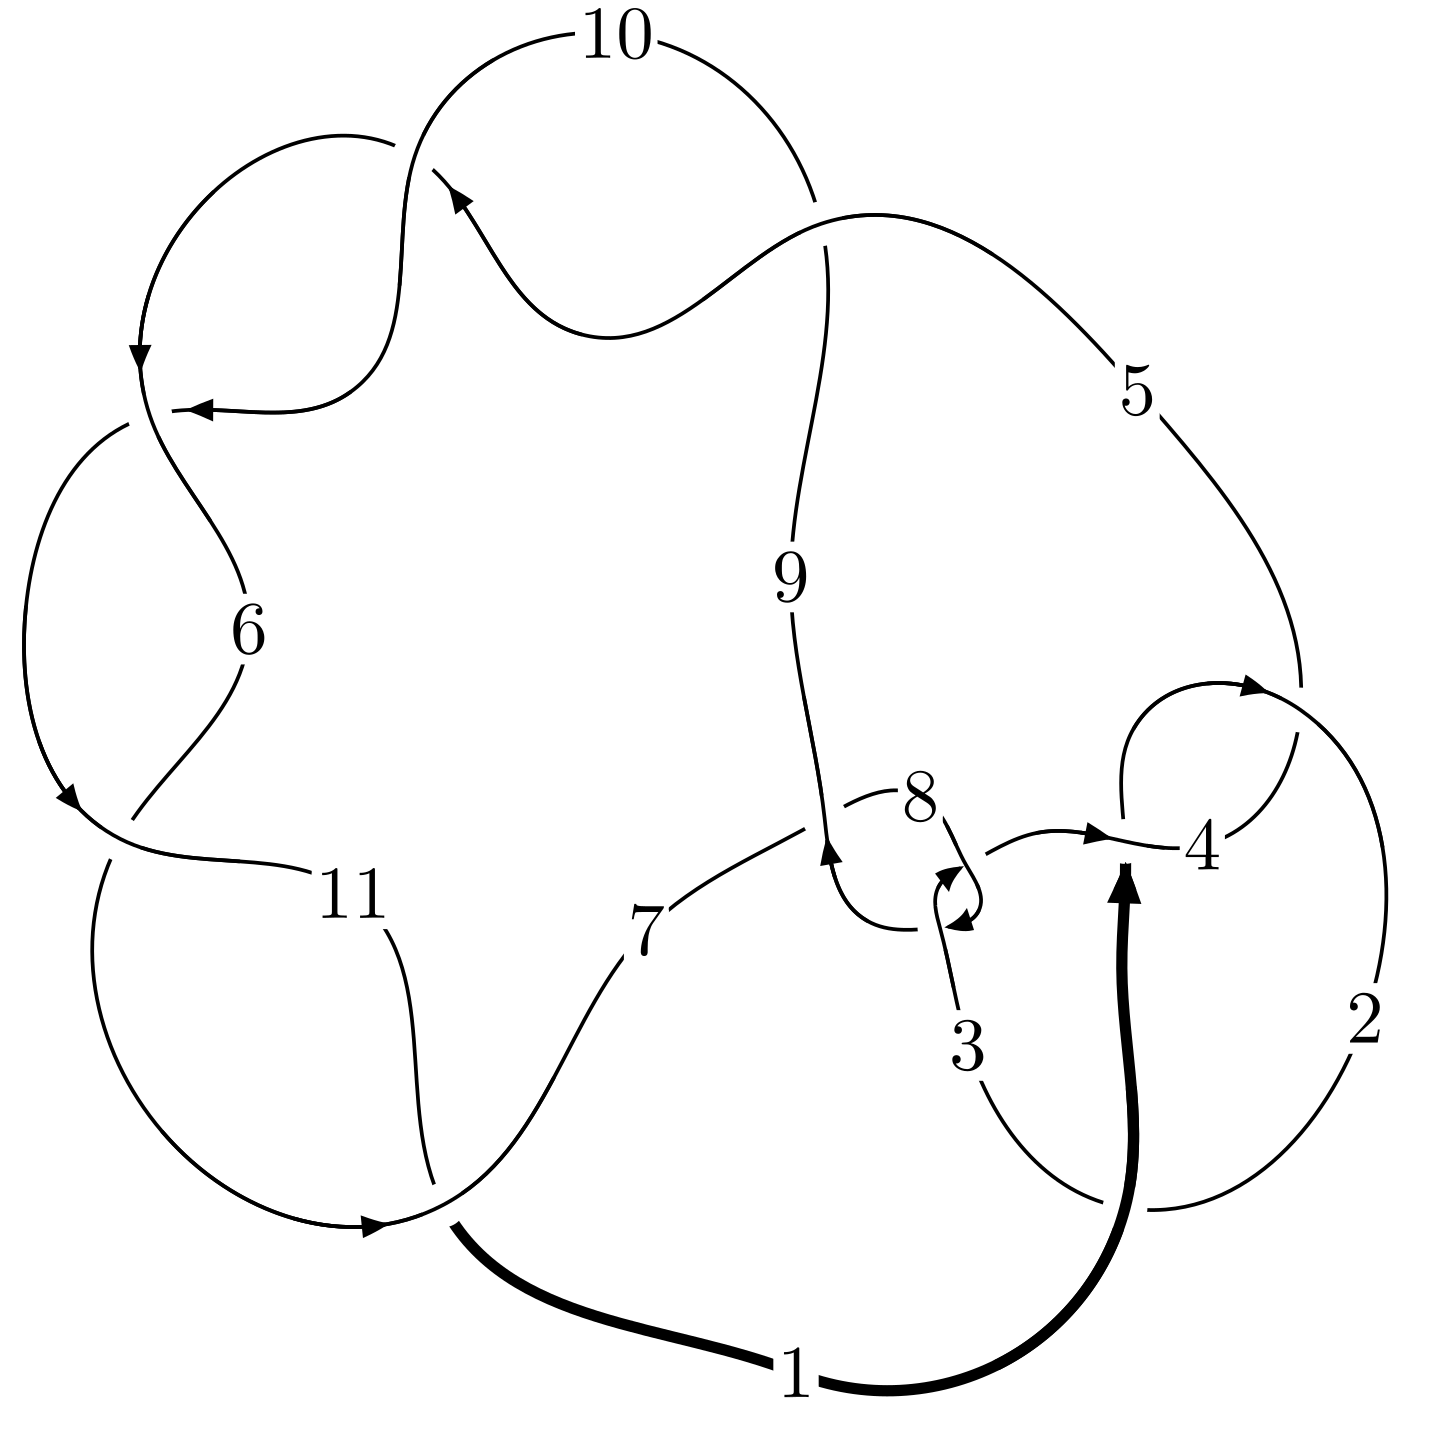
\includegraphics[width=112pt]{../../../GIT/diagram.site/Diagrams/png/304_11a_55.png}\\
\ \ \ A knot diagram\footnotemark}&
\allowdisplaybreaks
\textbf{Linearized knot diagam} \\
\cline{2-2}
 &
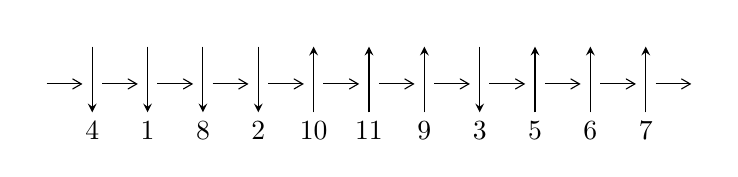
\begin{tikzpicture}[x=20pt, y=17pt]
	% nodes
	\node (C0) at (0, 0) {};
	\node (C1) at (1, 0) {};
	\node (C1U) at (1, +1) {};
	\node (C1D) at (1, -1) {4};

	\node (C2) at (2, 0) {};
	\node (C2U) at (2, +1) {};
	\node (C2D) at (2, -1) {1};

	\node (C3) at (3, 0) {};
	\node (C3U) at (3, +1) {};
	\node (C3D) at (3, -1) {8};

	\node (C4) at (4, 0) {};
	\node (C4U) at (4, +1) {};
	\node (C4D) at (4, -1) {2};

	\node (C5) at (5, 0) {};
	\node (C5U) at (5, +1) {};
	\node (C5D) at (5, -1) {10};

	\node (C6) at (6, 0) {};
	\node (C6U) at (6, +1) {};
	\node (C6D) at (6, -1) {11};

	\node (C7) at (7, 0) {};
	\node (C7U) at (7, +1) {};
	\node (C7D) at (7, -1) {9};

	\node (C8) at (8, 0) {};
	\node (C8U) at (8, +1) {};
	\node (C8D) at (8, -1) {3};

	\node (C9) at (9, 0) {};
	\node (C9U) at (9, +1) {};
	\node (C9D) at (9, -1) {5};

	\node (C10) at (10, 0) {};
	\node (C10U) at (10, +1) {};
	\node (C10D) at (10, -1) {6};

	\node (C11) at (11, 0) {};
	\node (C11U) at (11, +1) {};
	\node (C11D) at (11, -1) {7};
	\node (C12) at (12, 0) {};

	% arrows
	\draw[->,>={angle 60}]
	(C0) edge (C1) (C1) edge (C2) (C2) edge (C3) (C3) edge (C4) (C4) edge (C5) (C5) edge (C6) (C6) edge (C7) (C7) edge (C8) (C8) edge (C9) (C9) edge (C10) (C10) edge (C11) (C11) edge (C12) ;	\draw[->,>=stealth]
	(C1U) edge (C1D) (C2U) edge (C2D) (C3U) edge (C3D) (C4U) edge (C4D) (C5D) edge (C5U) (C6D) edge (C6U) (C7D) edge (C7U) (C8U) edge (C8D) (C9D) edge (C9U) (C10D) edge (C10U) (C11D) edge (C11U) ;
	\end{tikzpicture} \\
\hhline{~~} \\& 
\textbf{Solving Sequence} \\ \cline{2-2} 
 &
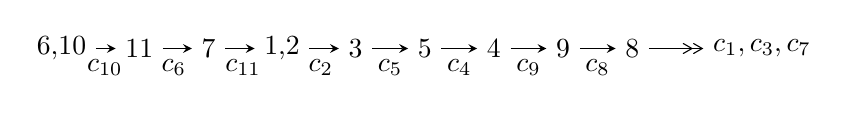
\begin{tikzpicture}[x=25pt, y=7pt]
	% node
	\node (A0) at (-1/8, 0) {6,10};
	\node (A1) at (1, 0) {11};
	\node (A2) at (2, 0) {7};
	\node (A3) at (49/16, 0) {1,2};
	\node (A4) at (33/8, 0) {3};
	\node (A5) at (41/8, 0) {5};
	\node (A6) at (49/8, 0) {4};
	\node (A7) at (57/8, 0) {9};
	\node (A8) at (65/8, 0) {8};
	\node (C1) at (1/2, -1) {$c_{10}$};
	\node (C2) at (3/2, -1) {$c_{6}$};
	\node (C3) at (5/2, -1) {$c_{11}$};
	\node (C4) at (29/8, -1) {$c_{2}$};
	\node (C5) at (37/8, -1) {$c_{5}$};
	\node (C6) at (45/8, -1) {$c_{4}$};
	\node (C7) at (53/8, -1) {$c_{9}$};
	\node (C8) at (61/8, -1) {$c_{8}$};
	\node (A9) at (10, 0) {$c_{1},c_{3},c_{7}$};

	% edge
	\draw[->,>=stealth]	
	(A0) edge (A1) (A1) edge (A2) (A2) edge (A3) (A3) edge (A4) (A4) edge (A5) (A5) edge (A6) (A6) edge (A7) (A7) edge (A8) ;
	\draw[->>,>={angle 60}]	
	(A8) edge (A9);
\end{tikzpicture} \\ 

\end{tabular} \\

\footnotetext{
The image of knot diagram is generated by the software ``\textbf{Draw programme}" developed by Andrew Bartholomew(\url{http://www.layer8.co.uk/maths/draw/index.htm\#Running-draw}), where we modified some parts for our purpose(\url{https://github.com/CATsTAILs/LinksPainter}).
}\phantom \\ \newline 
\centering \textbf{Ideals for irreducible components\footnotemark of $X_{\text{par}}$} 
 
\begin{align*}
I^u_{1}&=\langle 
u^{36}-23 u^{34}+\cdots+b-1,\;- u^{36}+u^{35}+\cdots+a-2,\;u^{37}-2 u^{36}+\cdots+u+1\rangle \\
I^u_{2}&=\langle 
b,\;a- u-1,\;u^2+u-1\rangle \\
\\
\end{align*}
\raggedright * 2 irreducible components of $\dim_{\mathbb{C}}=0$, with total 39 representations.\\
\footnotetext{All coefficients of polynomials are rational numbers. But the coefficients are sometimes approximated in decimal forms when there is not enough margin.}
\newpage
\renewcommand{\arraystretch}{1}
\centering \section*{I. $I^u_{1}= \langle u^{36}-23 u^{34}+\cdots+b-1,\;- u^{36}+u^{35}+\cdots+a-2,\;u^{37}-2 u^{36}+\cdots+u+1 \rangle$}
\flushleft \textbf{(i) Arc colorings}\\
\begin{tabular}{m{7pt} m{180pt} m{7pt} m{180pt} }
\flushright $a_{6}=$&$\begin{pmatrix}0\\u\end{pmatrix}$ \\
\flushright $a_{10}=$&$\begin{pmatrix}1\\0\end{pmatrix}$ \\
\flushright $a_{11}=$&$\begin{pmatrix}1\\- u^2\end{pmatrix}$ \\
\flushright $a_{7}=$&$\begin{pmatrix}u\\- u^3+u\end{pmatrix}$ \\
\flushright $a_{1}=$&$\begin{pmatrix}- u^2+1\\u^4-2 u^2\end{pmatrix}$ \\
\flushright $a_{2}=$&$\begin{pmatrix}u^{36}- u^{35}+\cdots-7 u+2\\- u^{36}+23 u^{34}+\cdots-7 u^2+1\end{pmatrix}$ \\
\flushright $a_{3}=$&$\begin{pmatrix}2 u^{36}- u^{35}+\cdots-7 u+1\\-2 u^{36}+46 u^{34}+\cdots+u+2\end{pmatrix}$ \\
\flushright $a_{5}=$&$\begin{pmatrix}- u\\u\end{pmatrix}$ \\
\flushright $a_{4}=$&$\begin{pmatrix}u^{35}- u^{34}+\cdots+6 u-2\\- u^{26}+16 u^{24}+\cdots-5 u^2+2 u\end{pmatrix}$ \\
\flushright $a_{9}=$&$\begin{pmatrix}- u^2+1\\u^2\end{pmatrix}$ \\
\flushright $a_{8}=$&$\begin{pmatrix}- u^7+4 u^5-4 u^3+2 u\\u^7-3 u^5+u\end{pmatrix}$\\ \flushright $a_{8}=$&$\begin{pmatrix}- u^7+4 u^5-4 u^3+2 u\\u^7-3 u^5+u\end{pmatrix}$\\&\end{tabular}
\flushleft \textbf{(ii) Obstruction class $= -1$}\\~\\
\flushleft \textbf{(iii) Cusp Shapes $= -8 u^{36}+11 u^{35}+\cdots+32 u+1$}\\~\\
\newpage\renewcommand{\arraystretch}{1}
\flushleft \textbf{(iv) u-Polynomials at the component}\newline \\
\begin{tabular}{m{50pt}|m{274pt}}
Crossings & \hspace{64pt}u-Polynomials at each crossing \\
\hline $$\begin{aligned}c_{1},c_{4}\end{aligned}$$&$\begin{aligned}
&u^{37}-3 u^{36}+\cdots-2 u+1
\end{aligned}$\\
\hline $$\begin{aligned}c_{2}\end{aligned}$$&$\begin{aligned}
&u^{37}+19 u^{36}+\cdots+4 u+1
\end{aligned}$\\
\hline $$\begin{aligned}c_{3},c_{8}\end{aligned}$$&$\begin{aligned}
&u^{37}- u^{36}+\cdots+3 u^2+4
\end{aligned}$\\
\hline $$\begin{aligned}c_{5},c_{6},c_{9}\\c_{10},c_{11}\end{aligned}$$&$\begin{aligned}
&u^{37}-2 u^{36}+\cdots+u+1
\end{aligned}$\\
\hline $$\begin{aligned}c_{7}\end{aligned}$$&$\begin{aligned}
&u^{37}-15 u^{36}+\cdots-24 u+16
\end{aligned}$\\
\hline
\end{tabular}\\~\\
\newpage\renewcommand{\arraystretch}{1}
\flushleft \textbf{(v) Riley Polynomials at the component}\newline \\
\begin{tabular}{m{50pt}|m{274pt}}
Crossings & \hspace{64pt}Riley Polynomials at each crossing \\
\hline $$\begin{aligned}c_{1},c_{4}\end{aligned}$$&$\begin{aligned}
&y^{37}-19 y^{36}+\cdots+4 y-1
\end{aligned}$\\
\hline $$\begin{aligned}c_{2}\end{aligned}$$&$\begin{aligned}
&y^{37}+y^{36}+\cdots-44 y-1
\end{aligned}$\\
\hline $$\begin{aligned}c_{3},c_{8}\end{aligned}$$&$\begin{aligned}
&y^{37}+15 y^{36}+\cdots-24 y-16
\end{aligned}$\\
\hline $$\begin{aligned}c_{5},c_{6},c_{9}\\c_{10},c_{11}\end{aligned}$$&$\begin{aligned}
&y^{37}-48 y^{36}+\cdots+25 y-1
\end{aligned}$\\
\hline $$\begin{aligned}c_{7}\end{aligned}$$&$\begin{aligned}
&y^{37}+11 y^{36}+\cdots+7712 y-256
\end{aligned}$\\
\hline
\end{tabular}\\~\\
\newpage\flushleft \textbf{(vi) Complex Volumes and Cusp Shapes}
$$\begin{array}{c|c|c}  
\text{Solutions to }I^u_{1}& \I (\text{vol} + \sqrt{-1}CS) & \text{Cusp shape}\\
 \hline 
\begin{aligned}
u &= -0.957621 + 0.312318 I \\
a &= \phantom{-}0.073185 - 0.193326 I \\
b &= -0.598010 + 0.868889 I\end{aligned}
 & \phantom{-}3.73036 - 4.62550 I & \phantom{-}7.76738 + 4.90690 I \\ \hline\begin{aligned}
u &= -0.957621 - 0.312318 I \\
a &= \phantom{-}0.073185 + 0.193326 I \\
b &= -0.598010 - 0.868889 I\end{aligned}
 & \phantom{-}3.73036 + 4.62550 I & \phantom{-}7.76738 - 4.90690 I \\ \hline\begin{aligned}
u &= -0.949350 + 0.385280 I \\
a &= -0.633743 + 1.188910 I \\
b &= -0.19879 - 2.12627 I\end{aligned}
 & \phantom{-}1.18638 - 9.75247 I & \phantom{-}4.12651 + 8.53256 I \\ \hline\begin{aligned}
u &= -0.949350 - 0.385280 I \\
a &= -0.633743 - 1.188910 I \\
b &= -0.19879 + 2.12627 I\end{aligned}
 & \phantom{-}1.18638 + 9.75247 I & \phantom{-}4.12651 - 8.53256 I \\ \hline\begin{aligned}
u &= \phantom{-}0.883228 + 0.295441 I \\
a &= -0.51817 - 1.46272 I \\
b &= -0.41139 + 2.28971 I\end{aligned}
 & -0.53133 + 3.88210 I & \phantom{-}2.57643 - 5.18911 I \\ \hline\begin{aligned}
u &= \phantom{-}0.883228 - 0.295441 I \\
a &= -0.51817 + 1.46272 I \\
b &= -0.41139 - 2.28971 I\end{aligned}
 & -0.53133 - 3.88210 I & \phantom{-}2.57643 + 5.18911 I \\ \hline\begin{aligned}
u &= -1.092520 + 0.081336 I \\
a &= -0.138007 + 0.822702 I \\
b &= -0.51460 - 1.46532 I\end{aligned}
 & \phantom{-}6.20655 - 2.48097 I & \phantom{-}9.67939 + 3.72325 I \\ \hline\begin{aligned}
u &= -1.092520 - 0.081336 I \\
a &= -0.138007 - 0.822702 I \\
b &= -0.51460 + 1.46532 I\end{aligned}
 & \phantom{-}6.20655 + 2.48097 I & \phantom{-}9.67939 - 3.72325 I \\ \hline\begin{aligned}
u &= -0.821917 + 0.258796 I \\
a &= \phantom{-}1.54271 - 0.10934 I \\
b &= -0.128202 + 0.262204 I\end{aligned}
 & -1.03449 - 1.41041 I & \phantom{-}2.89217 + 4.96755 I \\ \hline\begin{aligned}
u &= -0.821917 - 0.258796 I \\
a &= \phantom{-}1.54271 + 0.10934 I \\
b &= -0.128202 - 0.262204 I\end{aligned}
 & -1.03449 + 1.41041 I & \phantom{-}2.89217 - 4.96755 I\\
 \hline 
 \end{array}$$\newpage$$\begin{array}{c|c|c}  
\text{Solutions to }I^u_{1}& \I (\text{vol} + \sqrt{-1}CS) & \text{Cusp shape}\\
 \hline 
\begin{aligned}
u &= \phantom{-}0.819155 + 0.099014 I \\
a &= \phantom{-}0.507337 + 0.293800 I \\
b &= -0.977537 - 0.679950 I\end{aligned}
 & \phantom{-}1.50853 + 0.14938 I & \phantom{-}6.45155 + 0.46456 I \\ \hline\begin{aligned}
u &= \phantom{-}0.819155 - 0.099014 I \\
a &= \phantom{-}0.507337 - 0.293800 I \\
b &= -0.977537 + 0.679950 I\end{aligned}
 & \phantom{-}1.50853 - 0.14938 I & \phantom{-}6.45155 - 0.46456 I \\ \hline\begin{aligned}
u &= \phantom{-}0.669935 + 0.434127 I \\
a &= \phantom{-}1.373890 + 0.079928 I \\
b &= \phantom{-}0.053060 - 0.300111 I\end{aligned}
 & -0.46634 - 2.82395 I & \phantom{-}2.81248 + 2.07751 I \\ \hline\begin{aligned}
u &= \phantom{-}0.669935 - 0.434127 I \\
a &= \phantom{-}1.373890 - 0.079928 I \\
b &= \phantom{-}0.053060 + 0.300111 I\end{aligned}
 & -0.46634 + 2.82395 I & \phantom{-}2.81248 - 2.07751 I \\ \hline\begin{aligned}
u &= \phantom{-}0.126557 + 0.616394 I \\
a &= -0.649911 - 0.790815 I \\
b &= \phantom{-}0.194995 - 1.112060 I\end{aligned}
 & -2.10926 + 6.36685 I & -0.76306 - 6.73734 I \\ \hline\begin{aligned}
u &= \phantom{-}0.126557 - 0.616394 I \\
a &= -0.649911 + 0.790815 I \\
b &= \phantom{-}0.194995 + 1.112060 I\end{aligned}
 & -2.10926 - 6.36685 I & -0.76306 + 6.73734 I \\ \hline\begin{aligned}
u &= \phantom{-}0.446224 + 0.376427 I \\
a &= \phantom{-}0.324362 - 0.529872 I \\
b &= -0.123832 - 0.626016 I\end{aligned}
 & \phantom{-}1.20413 + 1.03970 I & \phantom{-}6.27276 - 4.95197 I \\ \hline\begin{aligned}
u &= \phantom{-}0.446224 - 0.376427 I \\
a &= \phantom{-}0.324362 + 0.529872 I \\
b &= -0.123832 + 0.626016 I\end{aligned}
 & \phantom{-}1.20413 - 1.03970 I & \phantom{-}6.27276 + 4.95197 I \\ \hline\begin{aligned}
u &= \phantom{-}0.164699 + 0.507419 I \\
a &= \phantom{-}1.129790 - 0.016387 I \\
b &= \phantom{-}0.171879 - 0.083354 I\end{aligned}
 & \phantom{-}0.29596 + 1.82108 I & \phantom{-}2.47769 - 3.83748 I \\ \hline\begin{aligned}
u &= \phantom{-}0.164699 - 0.507419 I \\
a &= \phantom{-}1.129790 + 0.016387 I \\
b &= \phantom{-}0.171879 + 0.083354 I\end{aligned}
 & \phantom{-}0.29596 - 1.82108 I & \phantom{-}2.47769 + 3.83748 I\\
 \hline 
 \end{array}$$\newpage$$\begin{array}{c|c|c}  
\text{Solutions to }I^u_{1}& \I (\text{vol} + \sqrt{-1}CS) & \text{Cusp shape}\\
 \hline 
\begin{aligned}
u &= -0.041396 + 0.496138 I \\
a &= -0.92411 + 1.21544 I \\
b &= \phantom{-}0.418405 + 1.058430 I\end{aligned}
 & -3.33947 - 1.17576 I & -4.43128 + 1.03066 I \\ \hline\begin{aligned}
u &= -0.041396 - 0.496138 I \\
a &= -0.92411 - 1.21544 I \\
b &= \phantom{-}0.418405 - 1.058430 I\end{aligned}
 & -3.33947 + 1.17576 I & -4.43128 - 1.03066 I \\ \hline\begin{aligned}
u &= -1.59215 + 0.06066 I \\
a &= -0.579041 - 0.150932 I \\
b &= -0.047557 + 0.344022 I\end{aligned}
 & \phantom{-}7.10974 + 1.19498 I & \phantom{-0.000000 } 0 \\ \hline\begin{aligned}
u &= -1.59215 - 0.06066 I \\
a &= -0.579041 + 0.150932 I \\
b &= -0.047557 - 0.344022 I\end{aligned}
 & \phantom{-}7.10974 - 1.19498 I & \phantom{-0.000000 } 0 \\ \hline\begin{aligned}
u &= \phantom{-}1.67626 + 0.05941 I \\
a &= -0.503100 + 0.060196 I \\
b &= -0.271772 - 0.167857 I\end{aligned}
 & \phantom{-}7.80383 + 2.56815 I & \phantom{-0.000000 } 0 \\ \hline\begin{aligned}
u &= \phantom{-}1.67626 - 0.05941 I \\
a &= -0.503100 - 0.060196 I \\
b &= -0.271772 + 0.167857 I\end{aligned}
 & \phantom{-}7.80383 - 2.56815 I & \phantom{-0.000000 } 0 \\ \hline\begin{aligned}
u &= -1.68061 + 0.03427 I \\
a &= -1.41650 + 1.55888 I \\
b &= \phantom{-}1.66994 - 1.91855 I\end{aligned}
 & \phantom{-}10.43060 - 0.72718 I & \phantom{-0.000000 } 0 \\ \hline\begin{aligned}
u &= -1.68061 - 0.03427 I \\
a &= -1.41650 - 1.55888 I \\
b &= \phantom{-}1.66994 + 1.91855 I\end{aligned}
 & \phantom{-}10.43060 + 0.72718 I & \phantom{-0.000000 } 0 \\ \hline\begin{aligned}
u &= -1.68650 + 0.07280 I \\
a &= \phantom{-}0.09784 - 3.23140 I \\
b &= \phantom{-}0.52086 + 3.57531 I\end{aligned}
 & \phantom{-}8.52780 - 5.28278 I & \phantom{-0.000000 } 0 \\ \hline\begin{aligned}
u &= -1.68650 - 0.07280 I \\
a &= \phantom{-}0.09784 + 3.23140 I \\
b &= \phantom{-}0.52086 - 3.57531 I\end{aligned}
 & \phantom{-}8.52780 + 5.28278 I & \phantom{-0.000000 } 0\\
 \hline 
 \end{array}$$\newpage$$\begin{array}{c|c|c}  
\text{Solutions to }I^u_{1}& \I (\text{vol} + \sqrt{-1}CS) & \text{Cusp shape}\\
 \hline 
\begin{aligned}
u &= \phantom{-}1.70104 + 0.10270 I \\
a &= \phantom{-}0.45064 + 2.76832 I \\
b &= \phantom{-}0.21974 - 3.16301 I\end{aligned}
 & \phantom{-}10.4876 + 11.6846 I & \phantom{-0.000000 } 0 \\ \hline\begin{aligned}
u &= \phantom{-}1.70104 - 0.10270 I \\
a &= \phantom{-}0.45064 - 2.76832 I \\
b &= \phantom{-}0.21974 + 3.16301 I\end{aligned}
 & \phantom{-}10.4876 - 11.6846 I & \phantom{-0.000000 } 0 \\ \hline\begin{aligned}
u &= \phantom{-}1.70490 + 0.08169 I \\
a &= -0.92941 - 1.36566 I \\
b &= \phantom{-}1.13242 + 1.88410 I\end{aligned}
 & \phantom{-}13.1327 + 6.1887 I & \phantom{-0.000000 } 0 \\ \hline\begin{aligned}
u &= \phantom{-}1.70490 - 0.08169 I \\
a &= -0.92941 + 1.36566 I \\
b &= \phantom{-}1.13242 - 1.88410 I\end{aligned}
 & \phantom{-}13.1327 - 6.1887 I & \phantom{-0.000000 } 0 \\ \hline\begin{aligned}
u &= \phantom{-}1.73093 + 0.01518 I \\
a &= -0.67256 + 2.24479 I \\
b &= \phantom{-}1.13578 - 2.69126 I\end{aligned}
 & \phantom{-}16.2880 + 2.8364 I & \phantom{-0.000000 } 0 \\ \hline\begin{aligned}
u &= \phantom{-}1.73093 - 0.01518 I \\
a &= -0.67256 - 2.24479 I \\
b &= \phantom{-}1.13578 + 2.69126 I\end{aligned}
 & \phantom{-}16.2880 - 2.8364 I & \phantom{-0.000000 } 0 \\ \hline\begin{aligned}
u &= -0.201734\phantom{ +0.000000I} \\
a &= \phantom{-}3.92958\phantom{ +0.000000I} \\
b &= \phantom{-}0.509239\phantom{ +0.000000I}\end{aligned}
 & -1.30402\phantom{ +0.000000I} & -9.26700\phantom{ +0.000000I}\\
 \hline 
 \end{array}$$\newpage\newpage\renewcommand{\arraystretch}{1}
\centering \section*{II. $I^u_{2}= \langle b,\;a- u-1,\;u^2+u-1 \rangle$}
\flushleft \textbf{(i) Arc colorings}\\
\begin{tabular}{m{7pt} m{180pt} m{7pt} m{180pt} }
\flushright $a_{6}=$&$\begin{pmatrix}0\\u\end{pmatrix}$ \\
\flushright $a_{10}=$&$\begin{pmatrix}1\\0\end{pmatrix}$ \\
\flushright $a_{11}=$&$\begin{pmatrix}1\\u-1\end{pmatrix}$ \\
\flushright $a_{7}=$&$\begin{pmatrix}u\\- u+1\end{pmatrix}$ \\
\flushright $a_{1}=$&$\begin{pmatrix}u\\- u\end{pmatrix}$ \\
\flushright $a_{2}=$&$\begin{pmatrix}u+1\\0\end{pmatrix}$ \\
\flushright $a_{3}=$&$\begin{pmatrix}1\\u\end{pmatrix}$ \\
\flushright $a_{5}=$&$\begin{pmatrix}- u\\u\end{pmatrix}$ \\
\flushright $a_{4}=$&$\begin{pmatrix}1\\u\end{pmatrix}$ \\
\flushright $a_{9}=$&$\begin{pmatrix}u\\- u+1\end{pmatrix}$ \\
\flushright $a_{8}=$&$\begin{pmatrix}u\\- u+1\end{pmatrix}$\\ \flushright $a_{8}=$&$\begin{pmatrix}u\\- u+1\end{pmatrix}$\\&\end{tabular}
\flushleft \textbf{(ii) Obstruction class $= 1$}\\~\\
\flushleft \textbf{(iii) Cusp Shapes $= 5$}\\~\\
\newpage\renewcommand{\arraystretch}{1}
\flushleft \textbf{(iv) u-Polynomials at the component}\newline \\
\begin{tabular}{m{50pt}|m{274pt}}
Crossings & \hspace{64pt}u-Polynomials at each crossing \\
\hline $$\begin{aligned}c_{1}\end{aligned}$$&$\begin{aligned}
&(u-1)^2
\end{aligned}$\\
\hline $$\begin{aligned}c_{2},c_{4}\end{aligned}$$&$\begin{aligned}
&(u+1)^2
\end{aligned}$\\
\hline $$\begin{aligned}c_{3},c_{7},c_{8}\end{aligned}$$&$\begin{aligned}
&u^2
\end{aligned}$\\
\hline $$\begin{aligned}c_{5},c_{6}\end{aligned}$$&$\begin{aligned}
&u^2- u-1
\end{aligned}$\\
\hline $$\begin{aligned}c_{9},c_{10},c_{11}\end{aligned}$$&$\begin{aligned}
&u^2+u-1
\end{aligned}$\\
\hline
\end{tabular}\\~\\
\newpage\renewcommand{\arraystretch}{1}
\flushleft \textbf{(v) Riley Polynomials at the component}\newline \\
\begin{tabular}{m{50pt}|m{274pt}}
Crossings & \hspace{64pt}Riley Polynomials at each crossing \\
\hline $$\begin{aligned}c_{1},c_{2},c_{4}\end{aligned}$$&$\begin{aligned}
&(y-1)^2
\end{aligned}$\\
\hline $$\begin{aligned}c_{3},c_{7},c_{8}\end{aligned}$$&$\begin{aligned}
&y^2
\end{aligned}$\\
\hline $$\begin{aligned}c_{5},c_{6},c_{9}\\c_{10},c_{11}\end{aligned}$$&$\begin{aligned}
&y^2-3 y+1
\end{aligned}$\\
\hline
\end{tabular}\\~\\
\newpage\flushleft \textbf{(vi) Complex Volumes and Cusp Shapes}
$$\begin{array}{c|c|c}  
\text{Solutions to }I^u_{2}& \I (\text{vol} + \sqrt{-1}CS) & \text{Cusp shape}\\
 \hline 
\begin{aligned}
u &= \phantom{-}0.618034\phantom{ +0.000000I} \\
a &= \phantom{-}1.61803\phantom{ +0.000000I} \\
b &= \phantom{-0.000000 } 0\end{aligned}
 & -0.657974\phantom{ +0.000000I} & \phantom{-}5.00000\phantom{ +0.000000I} \\ \hline\begin{aligned}
u &= -1.61803\phantom{ +0.000000I} \\
a &= -0.618034\phantom{ +0.000000I} \\
b &= \phantom{-0.000000 } 0\end{aligned}
 & \phantom{-}7.23771\phantom{ +0.000000I} & \phantom{-}5.00000\phantom{ +0.000000I}\\
 \hline 
 \end{array}$$\newpage
\newpage\renewcommand{\arraystretch}{1}
\centering \section*{ III. u-Polynomials}
\begin{tabular}{m{50pt}|m{274pt}}
Crossings & \hspace{64pt}u-Polynomials at each crossing \\
\hline $$\begin{aligned}c_{1}\end{aligned}$$&$\begin{aligned}
&((u-1)^2)(u^{37}-3 u^{36}+\cdots-2 u+1)
\end{aligned}$\\
\hline $$\begin{aligned}c_{2}\end{aligned}$$&$\begin{aligned}
&((u+1)^2)(u^{37}+19 u^{36}+\cdots+4 u+1)
\end{aligned}$\\
\hline $$\begin{aligned}c_{3},c_{8}\end{aligned}$$&$\begin{aligned}
&u^2(u^{37}- u^{36}+\cdots+3 u^2+4)
\end{aligned}$\\
\hline $$\begin{aligned}c_{4}\end{aligned}$$&$\begin{aligned}
&((u+1)^2)(u^{37}-3 u^{36}+\cdots-2 u+1)
\end{aligned}$\\
\hline $$\begin{aligned}c_{5},c_{6}\end{aligned}$$&$\begin{aligned}
&(u^2- u-1)(u^{37}-2 u^{36}+\cdots+u+1)
\end{aligned}$\\
\hline $$\begin{aligned}c_{7}\end{aligned}$$&$\begin{aligned}
&u^2(u^{37}-15 u^{36}+\cdots-24 u+16)
\end{aligned}$\\
\hline $$\begin{aligned}c_{9},c_{10},c_{11}\end{aligned}$$&$\begin{aligned}
&(u^2+u-1)(u^{37}-2 u^{36}+\cdots+u+1)
\end{aligned}$\\
\hline
\end{tabular}\newpage\renewcommand{\arraystretch}{1}
\centering \section*{ IV. Riley Polynomials}
\begin{tabular}{m{50pt}|m{274pt}}
Crossings & \hspace{64pt}Riley Polynomials at each crossing \\
\hline $$\begin{aligned}c_{1},c_{4}\end{aligned}$$&$\begin{aligned}
&((y-1)^2)(y^{37}-19 y^{36}+\cdots+4 y-1)
\end{aligned}$\\
\hline $$\begin{aligned}c_{2}\end{aligned}$$&$\begin{aligned}
&((y-1)^2)(y^{37}+y^{36}+\cdots-44 y-1)
\end{aligned}$\\
\hline $$\begin{aligned}c_{3},c_{8}\end{aligned}$$&$\begin{aligned}
&y^2(y^{37}+15 y^{36}+\cdots-24 y-16)
\end{aligned}$\\
\hline $$\begin{aligned}c_{5},c_{6},c_{9}\\c_{10},c_{11}\end{aligned}$$&$\begin{aligned}
&(y^2-3 y+1)(y^{37}-48 y^{36}+\cdots+25 y-1)
\end{aligned}$\\
\hline $$\begin{aligned}c_{7}\end{aligned}$$&$\begin{aligned}
&y^2(y^{37}+11 y^{36}+\cdots+7712 y-256)
\end{aligned}$\\
\hline
\end{tabular}
\vskip 2pc
\end{document}